% =====================================================================
%  Chapitre 3 -- Architecture d'un réseau convolutif
%  Partie a : la couche convolutive (canaux, tenseurs de poids, biais,
%             nombre de paramètres) et les fonctions d'activation
% =====================================================================
\section{Chapitre 3 --- Architecture d'un réseau convolutif}

\chapterslide{Chapitre 3}{Architecture d'un réseau convolutif}%
{6 h --- couche convolutive, activation, pooling, flatten, dense, softmax}%
{\textbf{Objectifs.} Décrire précisément une \textbf{couche convolutive} : canaux
d'entrée et de sortie, tenseurs de poids, biais. Savoir \textbf{compter les paramètres}
d'une couche. Choisir une \textbf{fonction d'activation} et justifier le rôle central de
ReLU. Comprendre le \textbf{pooling}, le \textbf{flatten}, les couches \textbf{denses}
et la \textbf{softmax}. Assembler le pipeline complet d'un CNN.}

\begin{frame}{Plan du chapitre}
\begin{columns}[t]
\begin{column}{0.48\textwidth}
\begin{kbox}[Les cinq temps de ce chapitre]
\begin{enumerate}
  \item La couche convolutive : canaux et poids.
  \item Compter les paramètres.
  \item Les fonctions d'activation : pourquoi ReLU.
  \item Pooling, flatten, couches denses.
  \item La softmax et le pipeline complet.
\end{enumerate}
\end{kbox}
\end{column}
\begin{column}{0.48\textwidth}
\begin{ebox}[Ce que vous saurez faire]
\begin{itemize}
  \item Calculer le nombre de paramètres d'une couche convolutive.
  \item Comparer ce coût à celui d'une couche dense.
  \item Justifier la non-linéarité et le choix de ReLU.
  \item Décrire le trajet d'une image, de l'entrée à la prédiction.
\end{itemize}
\end{ebox}
\end{column}
\end{columns}
\vspace{1mm}
\begin{wbox}[Une couche convolutive n'est pas « une boîte noire »]
Trois objets seulement : un \textbf{tenseur de poids} (les filtres appris),
un \textbf{vecteur de biais}, et la \textbf{convolution} qui les applique.
Le nombre de paramètres en découle par une formule exacte.
\end{wbox}
\end{frame}

\begin{frame}{De l'opération au bloc : la couche convolutive}
\begin{columns}[t]
\begin{column}{0.52\textwidth}
\begin{itemize}
  \item Le chapitre précédent : \emph{une} convolution avec \emph{un} noyau.
  \item Une couche convolutive applique \textbf{plusieurs} noyaux en parallèle.
  \item Chaque noyau produit \textbf{une carte d'activation} --- donc un
  \textbf{canal de sortie}.
  \item Une couche est donc définie par quatre nombres :
\end{itemize}
\begin{center}
\begin{tabular}{@{}ll@{}}
\toprule
\textbf{Symbole} & \textbf{Signification} \\
\midrule
$K$ & taille du noyau ($K \times K$) \\
$C_{\text{in}}$ & nombre de canaux d'entrée \\
$C_{\text{out}}$ & nombre de canaux de sortie \\
$b$ & biais, un par canal de sortie \\
\bottomrule
\end{tabular}
\end{center}
\end{column}
\begin{column}{0.44\textwidth}
\begin{kbox}[La sortie, pas à pas]
Une entrée $H \times W \times C_{\text{in}}$ passe par un glissement de
$C_{\text{out}}$ noyaux $K \times K$ : la sortie est un tenseur
$H' \times W' \times C_{\text{out}}$.

\medskip
Toutes les cartes d'un même canal partagent \textbf{un seul} jeu de poids :
c'est le partage de poids du chapitre 1, appliqué canal par canal.
\end{kbox}
\end{column}
\end{columns}
\end{frame}

\begin{frame}{Les canaux : entrée, sortie, et ce qu'ils représentent}
\begin{columns}[t]
\begin{column}{0.50\textwidth}
\begin{itemize}
  \item \textbf{Canal d'entrée} : une « profondeur » de l'entrée.
  Une image RVB a $C_{\text{in}} = 3$ ; une image grise, $C_{\text{in}} = 1$.
  \item \textbf{Canal de sortie} : produit par \emph{un} noyau. Sa carte
  d'activation indique \emph{où} le motif détecté apparaît.
  \item En profondeur, les canaux d'entrée deviennent eux-mêmes des cartes
  intermédiaires : un canal de sortie résume \textbf{tous} les canaux d'entrée.
\end{itemize}
\end{column}
\begin{column}{0.46\textwidth}
\begin{ebox}[Image du vocabulaire]
\begin{itemize}
  \item Entrée : l'image, ou les cartes issues de la couche précédente.
  \item Filtre (noyau) : un petit tenseur $K \times K \times C_{\text{in}}$.
  \item Carte d'activation : la réponse du filtre, plan spatial
  $H' \times W'$.
  \item Canal de sortie = une carte d'activation.
\end{itemize}
\end{ebox}
\end{column}
\end{columns}
\vspace{1mm}
\begin{kbox}[Point clé]
Le nombre de canaux de sortie est une \textbf{décision d'architecture}
(32, 64, 128 \dots), pas un résultat du calcul.
\end{kbox}
\end{frame}

\begin{frame}{Le tenseur de poids : combien de poids par filtre ?}
\begin{columns}[t]
\begin{column}{0.50\textwidth}
\begin{itemize}
  \item Un filtre doit lire \textbf{tous} les canaux d'entrée :
  il a la forme $K \times K \times C_{\text{in}}$.
  \item Donc $K^2 \times C_{\text{in}}$ poids \emph{par filtre}.
  \item Et comme il y a $C_{\text{out}}$ filtres, la couche possède
  $K^2 \times C_{\text{in}} \times C_{\text{out}}$ poids.
\end{itemize}
\begin{kbox}[Le tenseur de poids, vu comme une pile]
$C_{\text{out}}$ filtres, chacun empilant $C_{\text{in}}$ noyaux $K \times K$.
Plutôt que de sommer les canaux à la main, la pile les traite d'un coup.
\end{kbox}
\end{column}
\begin{column}{0.46\textwidth}
\begin{wbox}[Ne pas oublier le biais]
À chaque canal de sortie correspond \textbf{un} biais (un scalaire décalé
après la somme des produits). Il y en a donc $C_{\text{out}}$.
\end{wbox}
\begin{ebox}[Nombre de paramètres d'une couche conv]
\[
\boxed{\,P = K^2 \times C_{\text{in}} \times C_{\text{out}} + C_{\text{out}}\,}
\]
Les biais sont facultatifs (\py{bias=False}) mais presque toujours présents.
\end{ebox}
\end{column}
\end{columns}
\end{frame}

\begin{frame}{Trois exemples chiffrés}
\begin{center}
\begin{tabular}{@{}lccc@{}}
\toprule
\textbf{Couche} & \textbf{Calcul} & \textbf{Paramètres} \\
\midrule
$3\times 3$, $C_{\text{in}}=1 \to C_{\text{out}}=32$
  & $3^2 \times 1 \times 32 + 32$ & $= 320$ \\
$3\times 3$, $C_{\text{in}}=3 \to C_{\text{out}}=64$
  & $3^2 \times 3 \times 64 + 64$ & $= 1\,792$ \\
$3\times 3$, $C_{\text{in}}=64 \to C_{\text{out}}=128$
  & $3^2 \times 64 \times 128 + 128$ & $= 73\,856$ \\
\bottomrule
\end{tabular}
\end{center}
\vspace{1.5mm}
\begin{columns}[t]
\begin{column}{0.48\textwidth}
\begin{ebox}[Lecture des résultats]
Passer de 1 à 3 canaux d'entrée triple presque les poids ($320 \to 1\,792$) ;
passer de 3 à 64 canaux d'entrée les multiplie par plus de $40$
($1\,792 \to 73\,856$). Le coût croît \textbf{linéairement} en
$C_{\text{in}} \times C_{\text{out}}$.
\end{ebox}
\end{column}
\begin{column}{0.48\textwidth}
\begin{kbox}[Un repère]
Une couche $3\times 3$ en $64 \to 128$ coûte $73\,856$ paramètres : bien
moins qu'une seule matrice dense $1\,024 \to 1\,000$, qui en compte
\textbf{1\,025\,000}. La convolution reste \emph{économe}.
\end{kbox}
\end{column}
\end{columns}
\end{frame}

\begin{frame}{Ce que représentent les paramètres}
\begin{center}
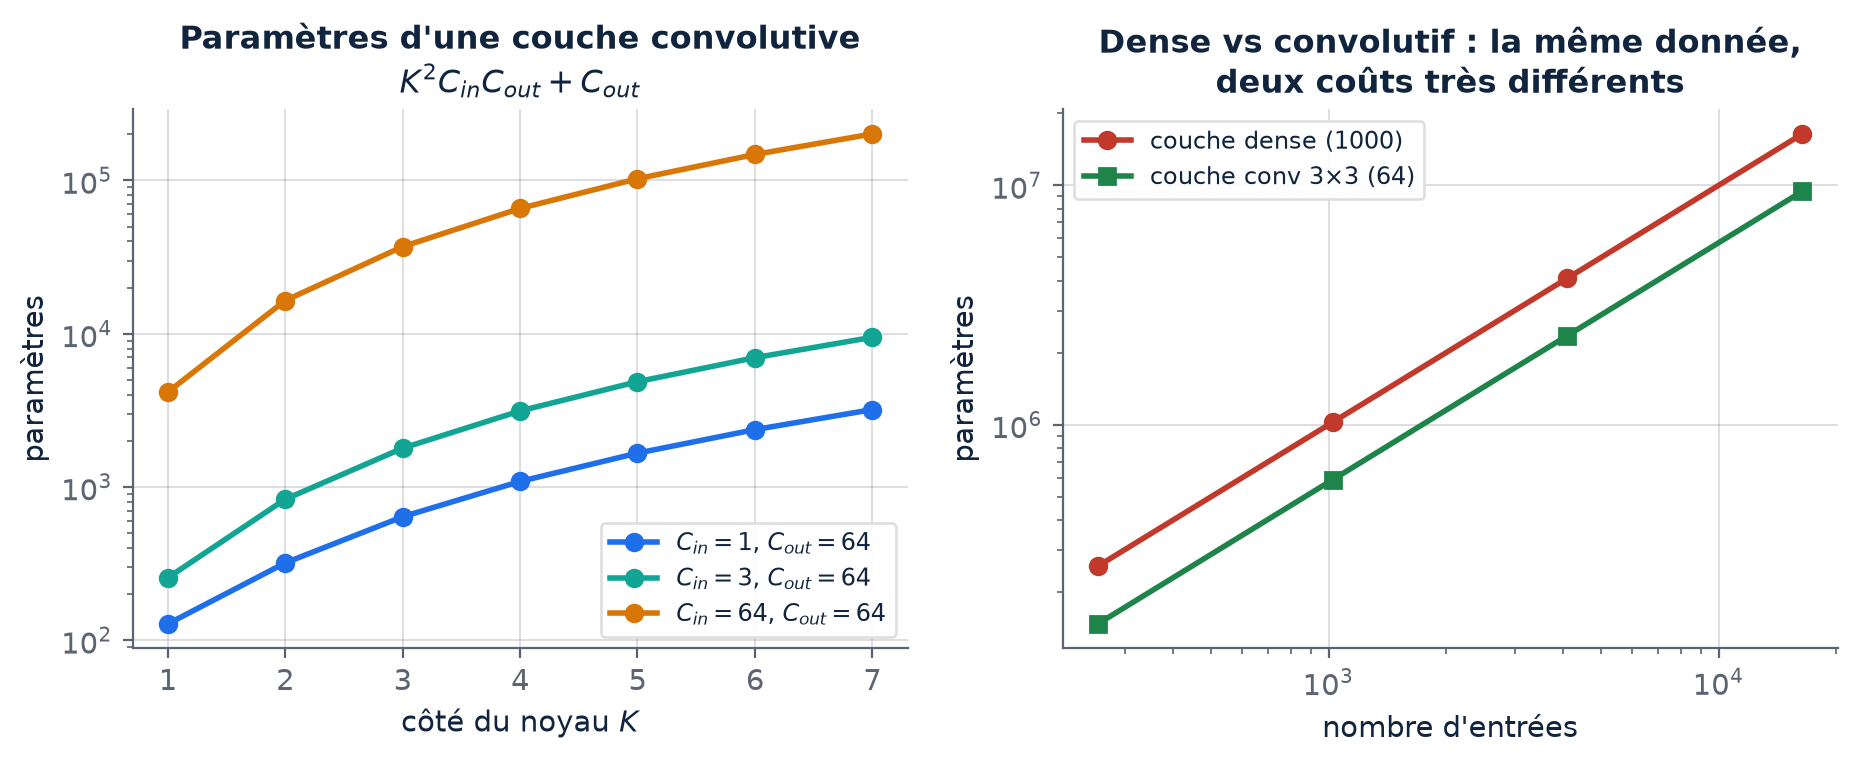
\includegraphics[width=0.80\textwidth]{h01_parametres_couches.png}
\end{center}
\vspace{1mm}
\begin{kbox}[À retenir de la figure]
Le nombre de paramètres d'une couche convolutive ne dépend \textbf{pas de la
taille de l'image}, mais seulement de la taille du noyau et du nombre de
canaux. C'est ce découplage qui rend les CNN utilisables sur de grandes images.
\end{kbox}
\end{frame}

\begin{frame}{Convolution contre couche dense}
\begin{columns}[t]
\begin{column}{0.50\textwidth}
\begin{wbox}[Le mur du dense]
Une couche dense reliant deux tenseurs « aplatis » connecte \emph{chaque}
entrée à \emph{chaque} sortie. Son coût explose avec la résolution.
\end{wbox}
\begin{itemize}
  \item La couche conv partage le \textbf{même} filtre partout.
  \item Elle ne regarde qu'un \textbf{voisinage local}.
  \item Résultat : ordres de grandeur en moins de paramètres.
\end{itemize}
\end{column}
\begin{column}{0.46\textwidth}
\begin{center}
\begin{tabular}{@{}lcc@{}}
\toprule
& \textbf{Conv} & \textbf{Dense} \\
\midrule
Poids liés à la position & non & oui \\
Partage de poids & oui & non \\
Dépend de la résolution & non & oui \\
Structure spatiale & conservée & perdue \\
\bottomrule
\end{tabular}
\end{center}
\begin{kbox}[La bonne lecture]
On ne remplace pas le dense : on l'\textbf{utilise à la fin}, quand la
structure spatiale a été résumée.
\end{kbox}
\end{column}
\end{columns}
\end{frame}

\begin{frame}[fragile]{Compter les paramètres en Python}
\begin{columns}[t]
\begin{column}{0.54\textwidth}
\begin{codebox}[Deux couches dans PyTorch]
\begin{lstlisting}
import torch.nn as nn

conv1 = nn.Conv2d(in_channels=3, out_channels=64, kernel_size=3)
conv2 = nn.Conv2d(in_channels=64, out_channels=128, kernel_size=3)

def nb_p(c):
    return sum(p.numel() for p in c.parameters())

print(nb_p(conv1))   # 3*3*3*64 + 64
print(nb_p(conv2))   # 3*3*64*128 + 128
\end{lstlisting}
\end{codebox}
\end{column}
\begin{column}{0.44\textwidth}
\begin{ebox}[Sortie attendue]
\py{conv1} : $3^2 \times 3 \times 64 + 64 = 1\,792$ paramètres.

\medskip
\py{conv2} : $3^2 \times 64 \times 128 + 128 = 73\,856$ paramètres.
\end{ebox}
\begin{kbox}[Vérification utile]
Compter les paramètres « à la main » puis avec \py{numel()} : l'accord des
deux valeurs est le meilleur test de la formule.
\end{kbox}
\end{column}
\end{columns}
\end{frame}

\begin{frame}{Il manque une pièce : la non-linéarité}
\begin{columns}[t]
\begin{column}{0.52\textwidth}
\begin{wbox}[Empiler des convolutions reste linéaire]
La convolution est une opération \textbf{linéaire}. Empiler deux couches
conv sans activation équivaut à \emph{une seule} convolution équivalente.
Un réseau purement convolutif ne pourrait donc apprendre que des relations
linéaires.
\end{wbox}
\begin{itemize}
  \item L'activation \textbf{casse la linéarité} entre deux couches.
  \item C'est elle qui permet la \textbf{hiérarchie} : bords, puis motifs,
  puis objets.
  \item Elle s'applique \emph{après} la convolution, élément par élément.
\end{itemize}
\end{column}
\begin{column}{0.44\textwidth}
\begin{kbox}[Sans activation, pas de profondeur]
\begin{center}
conv $\to$ conv $\;\equiv\;$ conv
\end{center}
Ajouter des couches n'augmente alors \emph{pas} la capacité de représentation.
La fonction d'activation est ce qui donne un sens à la profondeur.
\end{kbox}
\end{column}
\end{columns}
\end{frame}

\begin{frame}{ReLU : la fonction d'activation de référence}
\begin{columns}[t]
\begin{column}{0.50\textwidth}
\[
\mathrm{ReLU}(x) = \max(0,\, x)
\]
\begin{itemize}
  \item Les valeurs négatives deviennent $0$ ; les positives sont inchangées.
  \item Calcul \textbf{trivial} (un test) : peu coûteux en temps machine.
  \item Sa dérivée est simple : $1$ si $x>0$, $0$ sinon.
\end{itemize}
\begin{ebox}[Exemples numériques]
$\mathrm{ReLU}(-3) = 0$ \qquad $\mathrm{ReLU}(0) = 0$ \qquad
$\mathrm{ReLU}(2{,}5) = 2{,}5$
\end{ebox}
\end{column}
\begin{column}{0.46\textwidth}
\begin{kbox}[Pourquoi elle convient aux CNN]
\begin{itemize}
  \item Pas de « saturation » pour les grandes valeurs positives : le
  gradient ne s'évanouit pas.
  \item Elle préserve un gradient fort là où le motif est présent.
  \item Elle crée une sortie \textbf{creuse} : peu de neurones actifs.
\end{itemize}
\end{kbox}
\end{column}
\end{columns}
\end{frame}

\begin{frame}{Les fonctions d'activation en une figure}
\begin{center}
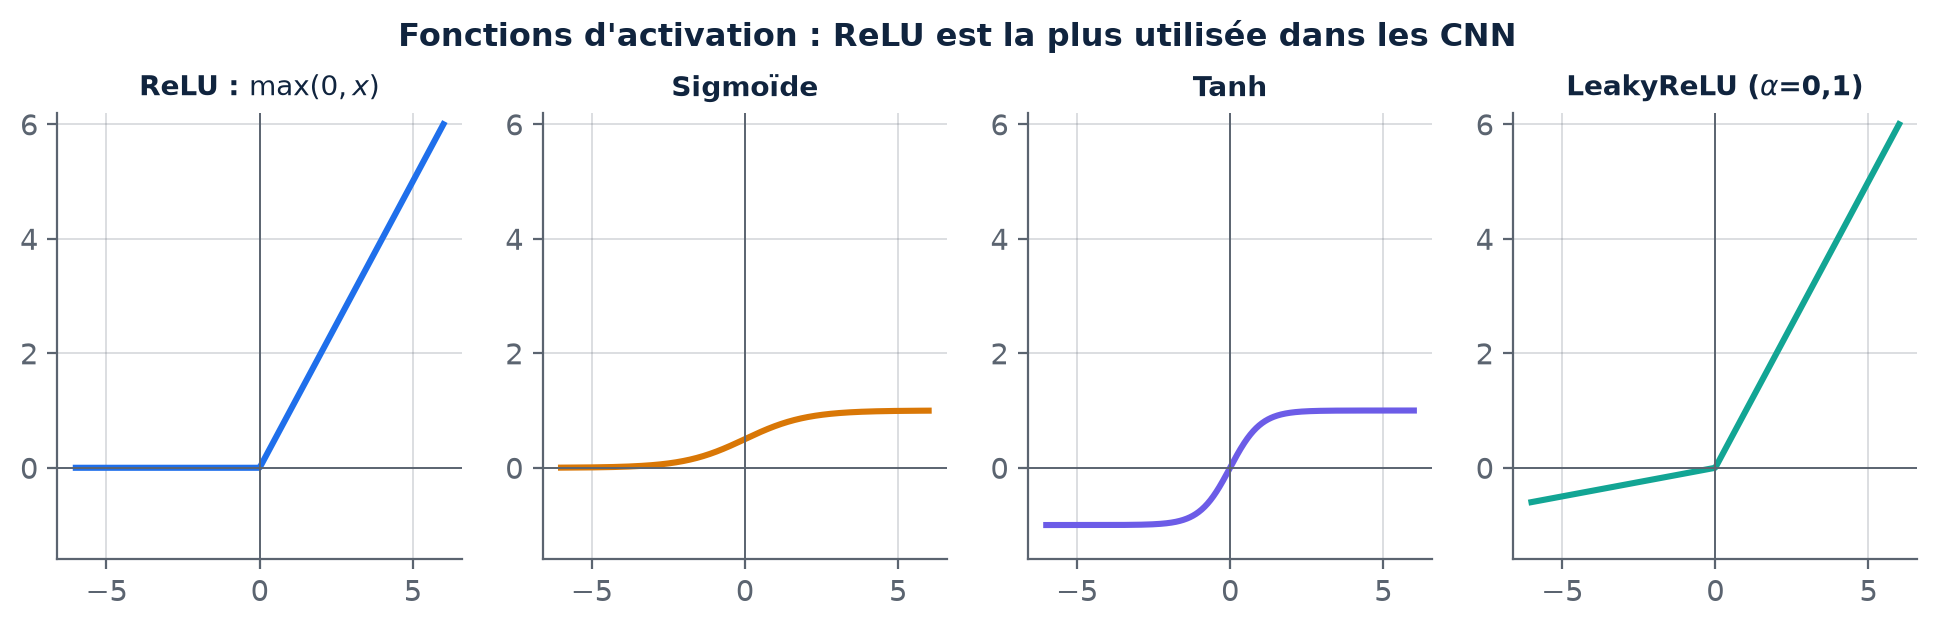
\includegraphics[width=0.90\textwidth]{h02_activations.png}
\end{center}
\vspace{1mm}
\begin{kbox}[Ce qu'il faut voir]
Chaque courbe transforme le score du neurone. ReLU est linéaire par morceaux,
la sigmoïde et la tangente hyperbolique sont des courbes en « S » qui
\textbf{saturent} aux extrémités : c'est là que leur gradient s'annule.
\end{kbox}
\end{frame}

\begin{frame}{Les variantes : sigmoïde, tanh, LeakyReLU}
\begin{columns}[t]
\begin{column}{0.52\textwidth}
\begin{center}
\begin{tabular}{@{}lll@{}}
\toprule
\textbf{Nom} & \textbf{Forme} & \textbf{Usage} \\
\midrule
Sigmoïde & $\dfrac{1}{1+e^{-x}}$ & sortie binaire \\
Tanh & $\dfrac{e^{x}-e^{-x}}{e^{x}+e^{-x}}$ & centrée en $0$ \\
ReLU & $\max(0,x)$ & défaut des CNN \\
LeakyReLU & $\max(\alpha x,x)$ & évite les morts \\
\bottomrule
\end{tabular}
\end{center}
\end{column}
\begin{column}{0.44\textwidth}
\begin{itemize}
  \item \textbf{Sigmoïde} : sortie dans $[0,1]$, mais saturation et gradient
  faible --- réservée aux dernières couches.
  \item \textbf{Tanh} : sortie dans $[-1,1]$, centrée ; gradient supérieur à
  la sigmoïde mais toujours saturant.
  \item \textbf{LeakyReLU} : petite pente $\alpha$ pour $x<0$, pour éviter
  qu'un neurone reste inactif.
\end{itemize}
\end{column}
\end{columns}
\vspace{1mm}
\begin{kbox}[Règle pratique]
Dans un CNN : \textbf{ReLU} dans les couches cachées, \textbf{softmax} et
sigmoïde à la sortie seulement.
\end{kbox}
\end{frame}

\begin{frame}{Pourquoi ReLU est devenue la norme}
\begin{columns}[t]
\begin{column}{0.31\textwidth}
\begin{ebox}[Dérivée constante]
Pour $x>0$, la dérivée vaut $1$ : le gradient traverse la couche sans être
atténué, même dans un réseau profond.
\end{ebox}
\end{column}
\begin{column}{0.31\textwidth}
\begin{ebox}[Coût de calcul]
Un simple \py{max(0, x)} --- pas d'exponentielle, pas de division. Négligeable
devant la convolution elle-même.
\end{ebox}
\end{column}
\begin{column}{0.31\textwidth}
\begin{ebox}[Convergence]
Les activations creuses accélèrent l'apprentissage et réduisent le
surapprentissage dans les premiers temps.
\end{ebox}
\end{column}
\end{columns}
\vspace{1mm}
\begin{wbox}[Le revers de ReLU]
Un neurone dont tous les scores deviennent négatifs peut rester bloqué à
$0$ : le gradient nul ne le réactive plus (problème des « neurones morts »).
LeakyReLU en atténue l'effet.
\end{wbox}
\end{frame}
